%=============================================================
% Session 23 – Deep Learning Course Notes
% Topic: Seq2Seq Stacked Layers + Bidirectional RNN + Hands-On
% Instructors: Prof. S R M Prasanna & Dr. Sunil Saumya
% Institution: IIIT Dharwad
% Date: February 9, 2026
%=============================================================

\documentclass[12pt,a4paper]{article}
\usepackage{amsmath,amsthm,amssymb,mathtools}
\usepackage{tikz}
\usetikzlibrary{arrows.meta,positioning,shapes.geometric,calc,fit,backgrounds}
\usepackage{graphicx}
\usepackage{booktabs,tabularx,multirow}
\usepackage[ruled,vlined,linesnumbered]{algorithm2e}
\usepackage[most]{tcolorbox}
\usepackage{hyperref}
\usepackage[capitalize,noabbrev]{cleveref}
\usepackage[margin=1in]{geometry}
\usepackage{fancyhdr}
\usepackage{enumitem}
\usepackage{xcolor}

%-------------------------------------------------------------
% tcolorbox environments
%-------------------------------------------------------------
\newtcolorbox{keyinsight}[1][]{colback=blue!5!white,colframe=blue!75!black,fonttitle=\bfseries,title=Key Insight,#1}
\newtcolorbox{example}[1][]{colback=green!5!white,colframe=green!75!black,fonttitle=\bfseries,title=Example,#1}
\newtcolorbox{warningbox}[1][]{colback=red!5!white,colframe=red!75!black,fonttitle=\bfseries,title=Warning,#1}

%-------------------------------------------------------------
% amsthm environments
%-------------------------------------------------------------
\newtheorem{theorem}{Theorem}[section]
\newtheorem{lemma}[theorem]{Lemma}
\newtheorem{definition}{Definition}[section]
\newtheorem{remark}{Remark}[section]

%-------------------------------------------------------------
% Header / Footer
%-------------------------------------------------------------
\pagestyle{fancy}
\fancyhf{}
\rhead{Session 23 -- Deep Learning}
\lhead{IIIT Dharwad}
\cfoot{\thepage}
\renewcommand{\headrulewidth}{0.4pt}

%-------------------------------------------------------------
% Colours
%-------------------------------------------------------------
\definecolor{codecolor}{rgb}{0.95,0.95,0.95}
\definecolor{lstblue}{rgb}{0.13,0.29,0.53}

%-------------------------------------------------------------
% Listings-style verbatim via tcolorbox
%-------------------------------------------------------------
\newtcolorbox{codebox}[1][]{colback=codecolor,colframe=gray!60,
  fonttitle=\ttfamily\small,title=#1,boxrule=0.5pt}

%-------------------------------------------------------------
% Metadata
%-------------------------------------------------------------
\title{\textbf{Deep Learning -- Session 23}\\[0.4em]
       \large Bidirectional RNN, Seq2Seq Stacked Layers, and Hands-On Implementation}
\author{Prof.\ S\,R\,M\,Prasanna \and Dr.\ Sunil Saumya\\[0.3em]
        \normalsize Indian Institute of Information Technology Dharwad}
\date{February 9, 2026 \quad (Deck: \texttt{05-DL-RNN} slide 74/109;
      \texttt{10-Seq2Seq} slides 6/25, 19/25)}

%=============================================================
\begin{document}
%=============================================================

\maketitle
\thispagestyle{fancy}

\begin{abstract}
Session 23 of the deep learning course covered three interconnected topics.
The session opened with the \emph{Bidirectional Recurrent Neural Network}
(Bi-RNN) architecture: two independent RNN (or LSTM/GRU) chains process the
input sequence in opposite directions, and each output position concatenates
the forward and backward hidden states, giving the network full past-and-future
context.  A recap of ``When Data is Sequential'' provided the RNN/LSTM/GRU
motivation within the Seq2Seq framing.  The stacked Seq2Seq architecture was
then detailed: multiple LSTM layers in both encoder and decoder increase model
capacity, with embedding layers at the input converting token IDs to dense
vectors.  The session concluded with a hands-on Google Colab walkthrough of an
English-to-Hindi machine translation pipeline --- covering tokenisation,
vocabulary construction, padding, teacher forcing, and the \texttt{Encoder}
class with a sanity check on output tensor shapes.
\end{abstract}

\newpage
\tableofcontents
\newpage

%=============================================================
\section{Introduction}
\label{sec:introduction}
%=============================================================

Recurrent Neural Networks in their simplest form process sequences strictly
from left to right.  While this \emph{unidirectional} assumption is natural for
causal prediction tasks (e.g., language modelling, real-time speech decoding),
many sequence labelling tasks benefit from knowing both the preceding and the
following context at each position.  This observation motivated the
\emph{Bidirectional RNN} (Bi-RNN)~\cite{schuster1997bidirectional}, which runs
two independent recurrent chains over the input: one in the standard
left-to-right direction, and one in the reverse right-to-left direction.

Complementing this architectural extension, \emph{Sequence-to-Sequence} (Seq2Seq)
models~\cite{sutskever2014sequence} address tasks where the output is itself a
variable-length sequence (e.g., machine translation, summarisation, question
answering).  Rather than a single recurrent network, Seq2Seq employs an
\emph{encoder} that compresses the source sequence into a fixed-size
\emph{context vector}, and a \emph{decoder} that generates the target sequence
auto-regressively from that context vector.

Session 23 unifies both threads.  After establishing the Bi-RNN formulation
(\cref{sec:birnn}), the session revisits the motivation for using recurrent
architectures with sequential data (\cref{sec:sequential}), then presents
stacked (deep) Seq2Seq models with embedding layers (\cref{sec:seq2seq}).
Finally, \cref{sec:handson} walks through the Google Colab implementation,
covering data preprocessing, tokenisation, padding, and the encoder module.

%=============================================================
\section{Background and Prerequisites}
\label{sec:background}
%=============================================================

\subsection{Vanilla Recurrent Neural Network}
\label{subsec:rnn_vanilla}

A Vanilla RNN processes a sequence $\mathbf{x} = (x_1, x_2, \ldots, x_T)$
step by step, maintaining a hidden state $h_t \in \mathbb{R}^d$ that summarises
all information seen up to time $t$:

\begin{equation}
  h_t = g\!\left(W_h\,h_{t-1} + W_x\,x_t + b\right),
  \label{eq:rnn_update}
\end{equation}

where $W_h \in \mathbb{R}^{d \times d}$, $W_x \in \mathbb{R}^{d \times n}$,
$b \in \mathbb{R}^{d}$, and $g$ is a non-linear activation (typically
$\tanh$).  The output at each time step is

\begin{equation}
  y_t = W_y\,h_t + b_y.
  \label{eq:rnn_output}
\end{equation}

\begin{remark}
  \label{rem:vanishing}
  Vanilla RNNs suffer from the \emph{vanishing gradient} problem for long
  sequences.  The gradient of the loss with respect to an early hidden state
  $h_1$ is a product of Jacobians, which tends to zero (or explodes)
  exponentially in $T$.
\end{remark}

\subsection{Long Short-Term Memory (LSTM)}
\label{subsec:lstm}

The LSTM~\cite{hochreiter1997long} mitigates the vanishing gradient by
introducing a \emph{cell state} $c_t$ and three gating mechanisms:

\begin{align}
  f_t   &= \sigma\!\left(W_f[h_{t-1}, x_t] + b_f\right),   \label{eq:lstm_f} \\
  i_t   &= \sigma\!\left(W_i[h_{t-1}, x_t] + b_i\right),   \label{eq:lstm_i} \\
  \tilde{c}_t &= \tanh\!\left(W_c[h_{t-1}, x_t] + b_c\right), \label{eq:lstm_c_tilde} \\
  c_t   &= f_t \odot c_{t-1} + i_t \odot \tilde{c}_t,       \label{eq:lstm_c} \\
  o_t   &= \sigma\!\left(W_o[h_{t-1}, x_t] + b_o\right),   \label{eq:lstm_o} \\
  h_t   &= o_t \odot \tanh(c_t).                            \label{eq:lstm_h}
\end{align}

\begin{keyinsight}
  The LSTM cell state $c_t$ flows through the network with only additive
  interactions, enabling gradients to propagate across many time steps without
  vanishing.  This property is crucial for long-sequence tasks such as machine
  translation.
\end{keyinsight}

\subsection{Gated Recurrent Unit (GRU)}
\label{subsec:gru}

The GRU~\cite{cho2014learning} simplifies LSTM by merging the forget and input
gates into a single \emph{update gate} $z_t$:

\begin{align}
  z_t &= \sigma\!\left(W_z[h_{t-1}, x_t]\right), \label{eq:gru_z} \\
  r_t &= \sigma\!\left(W_r[h_{t-1}, x_t]\right), \label{eq:gru_r} \\
  \tilde{h}_t &= \tanh\!\left(W[r_t \odot h_{t-1}, x_t]\right), \label{eq:gru_h_tilde} \\
  h_t &= (1 - z_t) \odot h_{t-1} + z_t \odot \tilde{h}_t. \label{eq:gru_h}
\end{align}

%=============================================================
\section{When Data is Sequential}
\label{sec:sequential}
%=============================================================

The slide ``When Data is Sequential: RNN / LSTM / GRU'' (Deck \texttt{10-Seq2Seq},
slide 6/25) distils the motivation for recurrent architectures into three
properties:

\begin{enumerate}[label=\textbf{P\arabic*.}]
  \item \textbf{Order matters.}  Changing the order of tokens in a sentence
        changes its meaning entirely.  A standard feed-forward network treats
        inputs as an unordered set.
  \item \textbf{Variable-length input.}  Natural language sentences, speech
        frames, and time-series windows differ in length.  RNNs handle arbitrary
        lengths naturally through weight sharing across time steps.
  \item \textbf{Context depends on previous elements.}  The hidden state
        $h_t$ in \cref{eq:rnn_update} acts as a running summary of all tokens
        seen so far, enabling the model to exploit long-range dependencies.
\end{enumerate}

\begin{figure}[h]
\centering
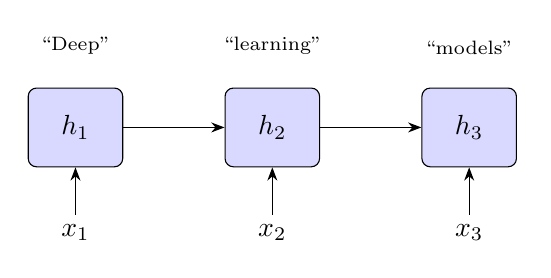
\begin{tikzpicture}[
  cell/.style={rectangle, draw, fill=blue!15, minimum width=1.2cm,
               minimum height=1.0cm, rounded corners=3pt},
  >=Stealth
]
  % Input tokens
  \node[cell] (h1) at (0,0)   {$h_1$};
  \node[cell] (h2) at (2.5,0) {$h_2$};
  \node[cell] (h3) at (5.0,0) {$h_3$};

  % Input arrows
  \node[below=0.6cm of h1] (x1) {$x_1$};
  \node[below=0.6cm of h2] (x2) {$x_2$};
  \node[below=0.6cm of h3] (x3) {$x_3$};
  \draw[->] (x1) -- (h1);
  \draw[->] (x2) -- (h2);
  \draw[->] (x3) -- (h3);

  % Recurrent arrows
  \draw[->] (h1) -- (h2);
  \draw[->] (h2) -- (h3);

  % Labels
  \node[above=0.3cm of h1, font=\scriptsize] {``Deep''};
  \node[above=0.3cm of h2, font=\scriptsize] {``learning''};
  \node[above=0.3cm of h3, font=\scriptsize] {``models''};
\end{tikzpicture}
\caption{Unidirectional RNN processing the sentence
         ``Deep learning models process sequences''.  The hidden state at each
         step summarises all preceding tokens.}
\label{fig:unidirectional_rnn}
\end{figure}

\begin{example}[title=Ambiguity Resolution with Context]
  Consider the sentence \emph{``I went to the bank to deposit money.''}
  At the moment of processing the word \emph{bank}, a left-to-right RNN
  has not yet seen \emph{``deposit money''}.  The word is ambiguous between
  a financial institution and a river bank.  If a right-to-left context is
  also available (carrying the information \emph{``deposit money''}), the
  ambiguity is resolved immediately.  This is precisely the motivation for
  Bidirectional RNNs.
\end{example}

\subsection{When Bidirectionality is Unsuitable}
\label{subsec:unsuitable}

Bidirectionality requires the \emph{complete} sequence to be available before
processing.  The following tasks are therefore unsuitable for Bi-RNNs:

\begin{itemize}
  \item \textbf{Next-word (language) modelling.}  At test time, the future
        tokens are not available; a backward pass cannot be computed.
        BERT (Bidirectional Encoder Representations from Transformers) addresses
        this by using a \emph{masked language modelling} objective instead of
        straightforward next-token prediction.
  \item \textbf{Online / streaming speech decoding.}  Speech signals evolve
        causally.  A backward pass would require buffering the entire utterance,
        introducing unacceptable latency.
\end{itemize}

\begin{keyinsight}
  The distinction between \emph{encoder}-type models (which can be
  bidirectional) and \emph{decoder}-type models (which must be causal) is
  central to the transformer literature.  BERT is a bidirectional encoder;
  GPT-style models are unidirectional decoders.
\end{keyinsight}

%=============================================================
\section{Bidirectional Recurrent Neural Networks}
\label{sec:birnn}
%=============================================================

\subsection{Architecture}
\label{subsec:birnn_arch}

A Bidirectional RNN runs two separate recurrent chains over the same input
sequence simultaneously:

\begin{enumerate}
  \item A \textbf{forward chain} processes tokens from $t=1$ to $t=T$,
        producing forward hidden states $\overrightarrow{h}_t$.
  \item A \textbf{backward chain} processes tokens from $t=T$ to $t=1$,
        producing backward hidden states $\overleftarrow{h}_t$.
\end{enumerate}

The output at position $t$ is the \emph{concatenation} of both states:

\begin{equation}
  y_t = \left[\overrightarrow{h}_t;\;\overleftarrow{h}_t\right]
        \in \mathbb{R}^{2d}.
  \label{eq:birnn_output}
\end{equation}

\cref{fig:birnn} illustrates the full architecture as shown in the lecture
slides (Deck \texttt{05-DL-RNN}, slide 74/109).

\begin{figure}[ht]
\centering
\begin{tikzpicture}[
  fwd/.style={rectangle, draw, fill=green!25, minimum width=1.1cm,
              minimum height=0.9cm, rounded corners=3pt, font=\small},
  bwd/.style={rectangle, draw, fill=orange!25, minimum width=1.1cm,
              minimum height=0.9cm, rounded corners=3pt, font=\small},
  out/.style={rectangle, draw, fill=gray!15, minimum width=1.1cm,
              minimum height=0.7cm, font=\scriptsize},
  >=Stealth, node distance=2.2cm
]
  % ---- Forward cells (bottom row) ----
  \node[fwd] (A0)  at (0,0)    {$A$};
  \node[fwd] (A1)  at (2.4,0)  {$A$};
  \node[fwd] (A2)  at (4.8,0)  {$A$};
  \node[fwd] (AT)  at (7.8,0)  {$A$};

  % ---- Backward cells (top row) ----
  \node[bwd] (B0)  at (0,2.2)   {$A'$};
  \node[bwd] (B1)  at (2.4,2.2) {$A'$};
  \node[bwd] (B2)  at (4.8,2.2) {$A'$};
  \node[bwd] (BT)  at (7.8,2.2) {$A'$};

  % ---- Inputs (below forward row) ----
  \foreach \i/\lbl in {0/$x_0$, 1/$x_1$, 2/$x_2$}{
    \pgfmathtruncatemacro{\xpos}{\i}
    \node[below=0.65cm of A\xpos] (x\i) {\lbl};
    \draw[->] (x\i) -- (A\xpos);
    \draw[->] (x\i) -- (B\xpos);
  }
  \node[below=0.65cm of AT] (xT) {$x_T$};
  \draw[->] (xT) -- (AT);
  \draw[->] (xT) -- (BT);

  % ---- Outputs (above backward row) ----
  \foreach \i in {0,1,2}{
    \node[out, above=0.65cm of B\i] (y\i) {$y_\i$};
    \draw[->] (B\i) -- (y\i);
    \draw[->] (A\i) -- (y\i);
  }
  \node[out, above=0.65cm of BT] (yT) {$y_T$};
  \draw[->] (BT) -- (yT);
  \draw[->] (AT) -- (yT);

  % ---- Forward recurrent arrows ----
  \draw[->] (A0) -- node[below,font=\scriptsize]{$s_0$} (A1);
  \draw[->] (A1) -- (A2);
  \draw[dashed,->] (A2) -- (AT);
  \node[left=0.5cm of A0, font=\scriptsize] {$s_0$};
  \node[right=0.4cm of AT, font=\scriptsize] {$s_T$};

  % ---- Backward recurrent arrows ----
  \draw[<-] (B0) -- node[above,font=\scriptsize]{} (B1);
  \draw[<-] (B1) -- (B2);
  \draw[dashed,<-] (B2) -- (BT);
  \node[left=0.5cm of B0, font=\scriptsize] {$s'_1$};
  \node[right=0.4cm of BT, font=\scriptsize] {$s'_0$};

  % ---- Ellipsis between A2/B2 and AT/BT ----
  \node at (6.3,0)   {\ldots};
  \node at (6.3,2.2) {\ldots};

  % ---- Legend ----
  \begin{scope}[shift={(0,-2.2)}]
    \node[fwd, minimum width=0.7cm] (lf) at (1,0) {$A$};
    \node[right=0.1cm of lf, font=\small] {Forward (left $\to$ right)};
    \node[bwd, minimum width=0.7cm] (lb) at (5,0) {$A'$};
    \node[right=0.1cm of lb, font=\small] {Backward (right $\to$ left)};
  \end{scope}
\end{tikzpicture}
\caption{Bidirectional RNN architecture (Deck \texttt{05-DL-RNN}, slide 74/109).
         Each output $y_t$ combines both forward and backward hidden states via
         concatenation.  Green cells ($A$) carry state left-to-right;
         orange cells ($A'$) carry state right-to-left.}
\label{fig:birnn}
\end{figure}

\subsection{Forward and Backward Equations}
\label{subsec:birnn_equations}

The forward and backward passes are independent recurrences sharing only the
input $x_t$:

\begin{align}
  \overrightarrow{h}_t &= g\!\left(
      W_{\overrightarrow{h}}\,\overrightarrow{h}_{t-1}
      + W_{\overrightarrow{x}}\,x_t + b_{\overrightarrow{h}}\right),
      \label{eq:birnn_fwd} \\[4pt]
  \overleftarrow{h}_t &= g\!\left(
      W_{\overleftarrow{h}}\,\overleftarrow{h}_{t+1}
      + W_{\overleftarrow{x}}\,x_t + b_{\overleftarrow{h}}\right).
      \label{eq:birnn_bwd}
\end{align}

Note the index difference: the forward state at $t$ depends on $t-1$, while
the backward state at $t$ depends on $t+1$.  The combined output is

\begin{equation}
  y_t = W_y\!\left[\overrightarrow{h}_t;\;\overleftarrow{h}_t\right] + b_y.
  \label{eq:birnn_combined}
\end{equation}

\begin{definition}
  \label{def:birnn}
  A \textbf{Bidirectional RNN} is a network consisting of two separate
  recurrent chains $\overrightarrow{\mathrm{RNN}}$ and
  $\overleftarrow{\mathrm{RNN}}$ that process the same input sequence in
  opposite temporal directions.  The output at each time step is a function of
  both chains' hidden states.
\end{definition}

\subsection{Deep Bidirectional RNNs}
\label{subsec:deep_birnn}

Just as feed-forward networks are deepened by stacking hidden layers, Bi-RNNs
can be stacked.  In a $L$-layer deep Bi-RNN:
\begin{itemize}
  \item Layer 1 receives the raw input $x_t$.
  \item Layer $\ell$ ($\ell > 1$) receives the output of layer $\ell-1$ at
        each time step $t$ as its input.
\end{itemize}

\begin{equation}
  h^{(\ell)}_t = \text{BiRNN}^{(\ell)}\!\left(h^{(\ell-1)}_t,\,
                   h^{(\ell-1)}_{t-1},\, h^{(\ell-1)}_{t+1}\right),
  \qquad \ell = 2, \ldots, L.
  \label{eq:deep_birnn}
\end{equation}

\begin{table}[ht]
\centering
\caption{Comparison of unidirectional and bidirectional RNN variants.}
\label{tab:rnn_comparison}
\begin{tabularx}{\textwidth}{lXXX}
\toprule
\textbf{Variant} & \textbf{Context Access} & \textbf{Typical Use Cases}
                 & \textbf{Limitations} \\
\midrule
Unidirectional RNN (L$\to$R) &
  Past context only &
  Language modelling, next-word prediction, online speech decoding &
  Cannot use future context \\
\addlinespace
Unidirectional RNN (R$\to$L) &
  Future context only &
  Right-to-left text generation &
  Cannot use past context \\
\addlinespace
Bidirectional RNN &
  Full past + future context &
  NER, POS tagging, sentiment analysis, fill-in-the-blank &
  Requires full sequence upfront; unsuitable for streaming \\
\addlinespace
Deep Bidirectional RNN &
  Hierarchical full context &
  Machine translation encoder, BERT-style pre-training &
  Requires full sequence; higher compute cost \\
\bottomrule
\end{tabularx}
\end{table}

%=============================================================
\section{Sequence-to-Sequence Models with Stacked Layers}
\label{sec:seq2seq}
%=============================================================

\subsection{Motivation: Variable-Length Output Sequences}
\label{subsec:seq2seq_motivation}

Classical RNN/LSTM models handle variable-length \emph{inputs} naturally.
Sequence-to-Sequence (Seq2Seq) models extend this to variable-length
\emph{outputs}.  The key distinction is captured by the following problem
statement.

\begin{definition}
  \label{def:seq2seq}
  Given a source sequence $\mathbf{x} = (x_1, \ldots, x_{T_x})$, a
  \textbf{Seq2Seq model} produces a target sequence
  $\mathbf{y} = (y_1, \ldots, y_{T_y})$ where $T_y$ is \emph{not} constrained
  to equal $T_x$.
\end{definition}

Applications include:
\begin{itemize}
  \item \textbf{Machine translation} (English $\to$ Hindi, etc.)
  \item \textbf{Text summarisation}
  \item \textbf{Question answering}
  \item \textbf{Speech recognition} (audio sequence $\to$ text sequence)
\end{itemize}

\subsection{Encoder--Decoder Architecture}
\label{subsec:enc_dec}

The canonical Seq2Seq model~\cite{sutskever2014sequence} consists of:

\begin{enumerate}
  \item An \textbf{Encoder} LSTM that reads the source sequence and produces a
        \emph{context vector} $\mathbf{c} = (h_{T_x}, c_{T_x})$ (the final
        hidden and cell states).
  \item A \textbf{Decoder} LSTM initialised with $\mathbf{c}$ that generates
        the target sequence auto-regressively:
\end{enumerate}

\begin{align}
  \mathbf{c} &= \text{Encoder}(x_1, \ldots, x_{T_x}), \label{eq:encoder} \\
  y_t &= \text{Decoder}(y_{t-1},\, \mathbf{c},\, h^d_{t-1}), \quad
         t = 1, \ldots, T_y. \label{eq:decoder}
\end{align}

\subsection{Embedding Layers}
\label{subsec:embedding}

Token IDs are high-dimensional, sparse one-hot vectors of dimensionality
$|\mathcal{V}|$ (vocabulary size).  An \emph{embedding layer} maps each token
index $i$ to a dense continuous vector:

\begin{equation}
  e_i = E \cdot \mathbf{1}_i \in \mathbb{R}^{d_e},
  \label{eq:embedding}
\end{equation}

where $E \in \mathbb{R}^{d_e \times |\mathcal{V}|}$ is a learnable embedding
matrix and $d_e \ll |\mathcal{V}|$.

\begin{keyinsight}
  Using an embedding layer instead of raw one-hot vectors provides two
  advantages: (1) the LSTM receives a \emph{semantically meaningful} dense
  representation of each token, and (2) the parameter count grows as
  $d_e \cdot |\mathcal{V}|$ rather than $|\mathcal{V}|^2$, which is far more
  efficient when the vocabulary is large.
\end{keyinsight}

\subsection{Stacked (Deep) Seq2Seq Architecture}
\label{subsec:stacked_seq2seq}

To increase model capacity, multiple LSTM layers can be stacked in both
encoder and decoder.  The architecture as presented in Deck \texttt{10-Seq2Seq}
(slide 19/25) is illustrated in \cref{fig:stacked_seq2seq}.

\begin{figure}[ht]
\centering
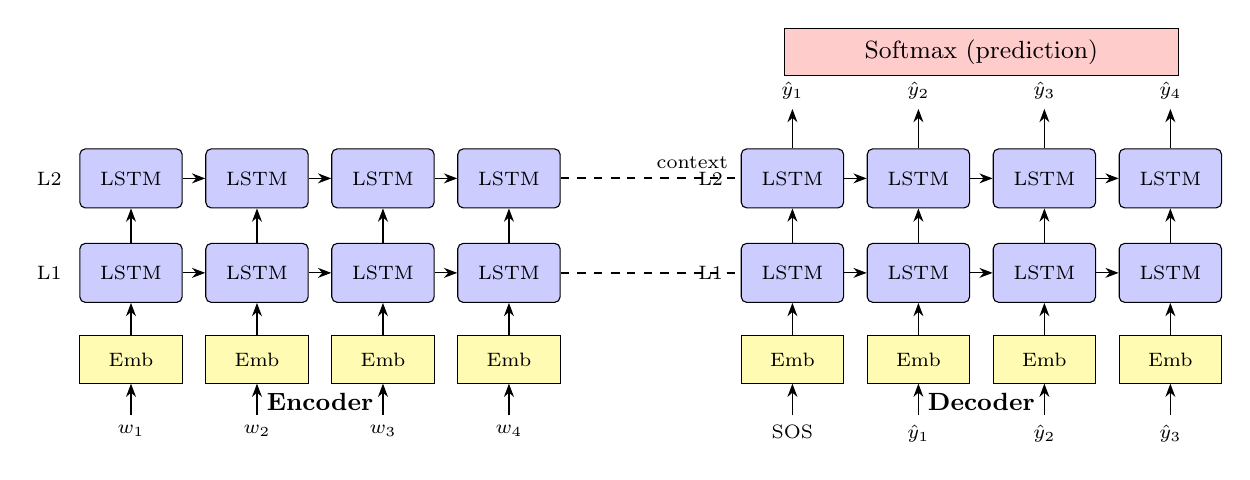
\begin{tikzpicture}[
  lstm/.style={rectangle, draw, fill=blue!20, minimum width=1.3cm,
               minimum height=0.75cm, font=\scriptsize, rounded corners=2pt},
  emb/.style={rectangle, draw, fill=yellow!30, minimum width=1.3cm,
              minimum height=0.6cm, font=\scriptsize},
  sm/.style={rectangle, draw, fill=red!20, minimum width=5cm,
             minimum height=0.6cm, font=\small},
  >=Stealth
]

  %--- ENCODER ---
  \begin{scope}
    % Layer 1
    \foreach \i/\x in {1/0, 2/1.6, 3/3.2, 4/4.8}{
      \node[lstm] (el1\i) at (\x, 0) {LSTM};
    }
    % Layer 2
    \foreach \i/\x in {1/0, 2/1.6, 3/3.2, 4/4.8}{
      \node[lstm] (el2\i) at (\x, 1.2) {LSTM};
    }
    % Embeddings
    \foreach \i/\x in {1/0, 2/1.6, 3/3.2, 4/4.8}{
      \node[emb]  (ee\i)  at (\x, -1.1) {Emb};
    }
    % Inputs
    \foreach \i/\x/\lbl in {1/0/$w_1$, 2/1.6/$w_2$, 3/3.2/$w_3$, 4/4.8/$w_4$}{
      \node[below=0.4cm of ee\i, font=\scriptsize] (ew\i) {\lbl};
      \draw[->] (ew\i) -- (ee\i);
      \draw[->] (ee\i) -- (el1\i);
      \draw[->] (el1\i) -- (el2\i);
    }
    % Recurrent L1
    \draw[->] (el11) -- (el12);
    \draw[->] (el12) -- (el13);
    \draw[->] (el13) -- (el14);
    % Recurrent L2
    \draw[->] (el21) -- (el22);
    \draw[->] (el22) -- (el23);
    \draw[->] (el23) -- (el24);
    % Label
    \node[left=0.1cm of el11, font=\scriptsize, rotate=0] {L1};
    \node[left=0.1cm of el21, font=\scriptsize] {L2};
    \node[below=1.4cm, font=\small\bfseries, xshift=2.4cm] {Encoder};
  \end{scope}

  %--- Context vector ---
  \draw[->, thick, dashed] (el24.east) to[out=0,in=180]
        node[above,font=\scriptsize, xshift=0.2cm]{context} (8.4, 1.2);
  \draw[->, thick, dashed] (el14.east) to[out=0,in=180] (8.4, 0);

  %--- DECODER ---
  \begin{scope}[xshift=8.4cm]
    % Layer 1
    \foreach \i/\x in {1/0, 2/1.6, 3/3.2, 4/4.8}{
      \node[lstm] (dl1\i) at (\x, 0) {LSTM};
    }
    % Layer 2
    \foreach \i/\x in {1/0, 2/1.6, 3/3.2, 4/4.8}{
      \node[lstm] (dl2\i) at (\x, 1.2) {LSTM};
    }
    % Embeddings
    \foreach \i/\x in {1/0, 2/1.6, 3/3.2, 4/4.8}{
      \node[emb]  (de\i)  at (\x, -1.1) {Emb};
    }
    % Inputs
    \foreach \i/\x/\lbl in {1/0/SOS, 2/1.6/$\hat{y}_1$, 3/3.2/$\hat{y}_2$, 4/4.8/$\hat{y}_3$}{
      \node[below=0.4cm of de\i, font=\scriptsize] (dw\i) {\lbl};
      \draw[->] (dw\i) -- (de\i);
      \draw[->] (de\i) -- (dl1\i);
      \draw[->] (dl1\i) -- (dl2\i);
    }
    % Recurrent L1
    \draw[->] (dl11) -- (dl12);
    \draw[->] (dl12) -- (dl13);
    \draw[->] (dl13) -- (dl14);
    % Recurrent L2
    \draw[->] (dl21) -- (dl22);
    \draw[->] (dl22) -- (dl23);
    \draw[->] (dl23) -- (dl24);
    % Output arrows
    \foreach \i in {1,2,3,4}{
      \node[above=0.5cm of dl2\i, font=\scriptsize] (do\i) {$\hat{y}_\i$};
      \draw[->] (dl2\i) -- (do\i);
    }
    % Softmax box
    \node[sm, above=1.3cm] at (2.4, 1.2) (sfm) {Softmax (prediction)};
    % Label
    \node[left=0.1cm of dl11, font=\scriptsize] {L1};
    \node[left=0.1cm of dl21, font=\scriptsize] {L2};
    \node[below=1.4cm, font=\small\bfseries, xshift=2.4cm] {Decoder};
  \end{scope}

\end{tikzpicture}
\caption{Stacked (deep) Seq2Seq architecture with embedding layers
         (Deck \texttt{10-Seq2Seq}, slide 19/25).  Both encoder and decoder
         use two LSTM layers.  The final context vectors from \emph{all} encoder
         layers initialise the corresponding decoder layers.}
\label{fig:stacked_seq2seq}
\end{figure}

\subsubsection*{Context Vector Propagation in Stacked Models}

A common question is whether context vectors from different encoder layers are
equivalent.  They are not.  In a 2-layer encoder:

\begin{align}
  h^{(1)}_t &= \text{LSTM}^{(1)}\!\left(e(x_t),\, h^{(1)}_{t-1}\right),
              \label{eq:enc_l1} \\
  h^{(2)}_t &= \text{LSTM}^{(2)}\!\left(h^{(1)}_t,\, h^{(2)}_{t-1}\right).
              \label{eq:enc_l2}
\end{align}

Layer 2 processes the \emph{transformed} representations from Layer 1 through
a different weight matrix $W^{(2)} \neq W^{(1)}$.  As a result, the context
vector from Layer 2 encodes a higher-level, more abstracted representation than
Layer 1's context vector, even though both are derived from the same source
sentence.

\begin{table}[ht]
\centering
\caption{Effect of architectural choices on Seq2Seq model performance
         (qualitative summary from lecture discussion).}
\label{tab:seq2seq_ablation}
\begin{tabularx}{\textwidth}{lXX}
\toprule
\textbf{Architecture Change} & \textbf{Benefit} & \textbf{Trade-off} \\
\midrule
Raw one-hot input (baseline) &
  Simple to implement &
  High-dimensional, sparse; no semantic similarity captured \\
\addlinespace
+ Embedding layer &
  Dense, learnable representations; semantic proximity captured &
  Additional parameters $d_e \times |\mathcal{V}|$; needs more data \\
\addlinespace
+ Stacked encoder (2 layers) &
  Hierarchical feature extraction; better long-range compression &
  More parameters; slower training \\
\addlinespace
+ Stacked decoder (2 layers) &
  Richer generation capacity &
  Context from \emph{all} encoder layers must initialise decoder layers \\
\addlinespace
+ Teacher forcing &
  Faster convergence during training; more stable gradients &
  Train/test discrepancy (exposure bias); only applicable at train time \\
\bottomrule
\end{tabularx}
\end{table}

\subsection{Limitations of the Basic Seq2Seq Model}
\label{subsec:seq2seq_limitations}

Despite its success, the encoder--decoder Seq2Seq model has two well-known
bottlenecks:

\begin{warningbox}
  \textbf{Context Vector Bottleneck.}  The entire source sequence must be
  compressed into a single fixed-size vector $\mathbf{c}$.  For long
  sentences (beyond $\approx$20--30 tokens), this representation becomes
  information-lossy: early and late words compete for representation in
  the limited vector dimensionality.
\end{warningbox}

\begin{enumerate}
  \item \textbf{Encoder-side bottleneck.}  All $T_x$ source tokens must be
        summarised into $\mathbf{c}$.  Important details from the beginning of
        a long paragraph may be overshadowed by more recent tokens due to the
        recency bias inherent in LSTM.
  \item \textbf{Decoder-side bottleneck.}  The same context vector (with minor
        variations from LSTM processing) is fed at every decoding step.  The
        decoder cannot selectively attend to the most relevant encoder states.
        For example, when generating the Hindi translation of ``I'', only the
        corresponding English token is relevant, not the entire source sentence.
\end{enumerate}

Both limitations are addressed by the \emph{attention mechanism}, which
allows the decoder to dynamically re-weight encoder hidden states at each
decoding step.  This mechanism is discussed in a subsequent session.

%=============================================================
\section{Training Seq2Seq Models: Teacher Forcing}
\label{sec:teacher_forcing}
%=============================================================

\subsection{Training Objective}
\label{subsec:training_obj}

During training, the model minimises the total cross-entropy loss summed over
all target tokens:

\begin{equation}
  \mathcal{L} = -\sum_{t=1}^{T_y} \log P(y_t \mid y_1, \ldots, y_{t-1},\,
                \mathbf{c};\,\theta).
  \label{eq:seq2seq_loss}
\end{equation}

\subsection{Teacher Forcing}
\label{subsec:teacher_forcing}

Without teacher forcing, the decoder receives its own predicted token
$\hat{y}_{t-1}$ as the input at step $t$.  Early in training, $\hat{y}_{t-1}$
is often wrong, causing the error to compound across decoding steps
(\emph{exposure bias}).

\textbf{Teacher forcing} substitutes the model's prediction with the
\emph{ground-truth} target token at each step:

\begin{equation}
  y_t = \text{Decoder}(y^*_{t-1},\, \mathbf{c},\, h^d_{t-1}),
  \label{eq:teacher_forcing}
\end{equation}

where $y^*_{t-1}$ is the ground-truth token at position $t-1$.

\begin{example}[title=Teacher Forcing for English-to-Hindi Translation]
  Suppose the source sentence is ``I am going'' and the target is
  ``Main ja raha hun.'' Without teacher forcing, if the decoder incorrectly
  predicts ``who'' as the first token, this wrong token propagates as input
  to the next step, compounding the error.  With teacher forcing, the correct
  token ``Main'' is fed at each step regardless of the model's prediction,
  enabling faster and more stable training convergence.
\end{example}

\begin{remark}
  \label{rem:teacher_forcing_inference}
  Teacher forcing is applied \emph{exclusively at training time}.  During
  inference (test time), the ground-truth sequence is unavailable, so the model
  operates auto-regressively: $\hat{y}_{t-1}$ is fed as input at step $t$.
\end{remark}

\begin{algorithm}[H]
\caption{Seq2Seq Training with Teacher Forcing}
\label{alg:seq2seq_train}
\SetAlgoLined
\KwIn{Source sequence $\mathbf{x}$, target sequence $\mathbf{y}^*$,
      model parameters $\theta$, learning rate $\eta$}
\KwOut{Updated parameters $\theta$}
\BlankLine
$\mathbf{c} = (h^e_{T_x}, c^e_{T_x}) \leftarrow \text{Encoder}(\mathbf{x};\,\theta_{\text{enc}})$\;
$h^d_0 \leftarrow h^e_{T_x}$,\quad $c^d_0 \leftarrow c^e_{T_x}$\;
$\mathcal{L} \leftarrow 0$\;
\For{$t = 1$ \KwTo $T_y$}{
  $\hat{y}_t,\, h^d_t,\, c^d_t \leftarrow
    \text{Decoder}\!\left(y^*_{t-1},\, h^d_{t-1},\, c^d_{t-1};\,
    \theta_{\text{dec}}\right)$\;
  $\mathcal{L} \leftarrow \mathcal{L} - \log P(y^*_t \mid \hat{y}_t)$\;
}
Back-propagate $\nabla_\theta \mathcal{L}$ through time\;
$\theta \leftarrow \theta - \eta \nabla_\theta \mathcal{L}$\;
\Return $\theta$\;
\end{algorithm}

%=============================================================
\section{Hands-On: Seq2Seq Implementation in PyTorch}
\label{sec:handson}
%=============================================================

The hands-on portion of Session 23 used
\texttt{dl-NTSeqToSeqModels.ipynb} (Google Colab) to build an
English-to-Hindi Seq2Seq pipeline from scratch.

\subsection{Dataset}
\label{subsec:dataset}

The dataset contains parallel English--Hindi sentence pairs sourced from
Kaggle (English-to-Hindi Machine Translation dataset).  Key statistics:

\begin{itemize}
  \item Total rows (after NaN removal): $\approx 1{,}77{,}006$.
  \item Training sample used in session: 10{,}000 rows (for computational
        tractability on a Colab CPU instance).
  \item Columns: \texttt{English sentence}, \texttt{Hindi sentence}.
\end{itemize}

\subsection{Data Preprocessing Pipeline}
\label{subsec:preprocessing}

The preprocessing pipeline follows five stages:

\begin{enumerate}
  \item \textbf{Data cleaning.}  Drop rows with missing values
        (\texttt{dropna}) and reset the index.
  \item \textbf{Type conversion.}  Convert each column to \texttt{str} and
        then to a list of token strings to handle mixed-type entries.
  \item \textbf{Tokenisation.}  Lowercase, strip whitespace, and split on
        spaces.
  \item \textbf{Vocabulary construction.}  Assign a unique integer index to
        each unique token.  Four special tokens are reserved:
        \texttt{PAD} (0), \texttt{UNK} (1), \texttt{SOS} (2), \texttt{EOS} (3).
  \item \textbf{Encoding.}  Map each sentence to a sequence of token indices.
        Hindi decoder sequences are prefixed with \texttt{SOS} and suffixed
        with \texttt{EOS}.
\end{enumerate}

\begin{codebox}[title=Tokenisation Function (Python)]
\begin{verbatim}
def tokenize(sentence):
    if not isinstance(sentence, str):
        return []
    return sentence.lower().strip().split()
\end{verbatim}
\end{codebox}

\subsubsection*{Vocabulary Sizes}

After processing 10{,}000 sentence pairs:
\begin{itemize}
  \item English vocabulary: $\approx 22{,}000$ unique tokens.
  \item Hindi vocabulary:   $\approx 24{,}000$ unique tokens.
\end{itemize}

The two vocabularies are entirely separate; the model uses the English
vocabulary at encode time and the Hindi vocabulary at decode time, so there is
no index collision.

\subsection{Padding for Batching}
\label{subsec:padding}

Because sentences in a batch differ in length, all sequences must be padded to
a common maximum length \texttt{MAX\_LEN} before being stacked into tensors.

\begin{codebox}[title=Padding Function (Python -- from slide V04)]
\begin{verbatim}
def pad_sequence(seq, max_len, pad_value=0):
    if len(seq) < max_len:
        seq = seq + [pad_value] * (max_len - len(seq))
    return seq

# Compute MAX_LEN across encoder and decoder sequences
MAX_LEN = max([len(s) for s in encoded_inputs])
MAX_LEN = max(MAX_LEN, max([len(s) for s in encoded_outputs]))
print("Max Sequence Length:", MAX_LEN)
\end{verbatim}
\end{codebox}

\begin{keyinsight}
  \texttt{MAX\_LEN} is computed as the maximum length \emph{across both encoder
  and decoder sequences}.  This ensures that the padding dimension is
  consistent for both the source and target batch tensors, which simplifies
  batching in the \texttt{DataLoader}.
\end{keyinsight}

The padding token index is 0 (\texttt{PAD}).  The model ignores padded
positions either through a padding mask or via PyTorch's
\texttt{pack\_padded\_sequence} utility, which avoids feeding padding tokens
to the LSTM.

\subsection{Encoder Implementation}
\label{subsec:encoder_impl}

The \texttt{Encoder} class wraps a single \texttt{nn.Embedding} layer followed
by an \texttt{nn.LSTM}:

\begin{codebox}[title=Encoder Hyperparameters and Instantiation (V05)]
\begin{verbatim}
EMBEDDING_DIM = 128
HIDDEN_DIM    = 256
ENCODER_DIM   = HIDDEN_DIM
DECODER_DIM   = HIDDEN_DIM

encoder = Encoder(
    input_dim    = len(encoder_vocab),
    embedding_dim = EMBEDDING_DIM,
    hidden_dim   = HIDDEN_DIM,
    n_layers     = 1,
    dropout      = 0
)
\end{verbatim}
\end{codebox}

\subsubsection*{Sanity Check}

After a forward pass on one batch from \texttt{train\_loader}:

\begin{codebox}[title=Encoder Sanity Check]
\begin{verbatim}
for src_batch, tgt_batch in train_loader:
    e_h, e_c = encoder(src_batch)
    print("e_h shape:", e_h.shape)  # torch.Size([1, 128, 256])
    print("e_c shape:", e_c.shape)  # torch.Size([1, 128, 256])
    break

# Remove layer dimension for decoder initialisation
context_h = e_h.squeeze(0)  # shape: [128, 256]
context_c = e_c.squeeze(0)  # shape: [128, 256]
\end{verbatim}
\end{codebox}

The output tensors have shape $[\texttt{n\_layers},\,\texttt{batch\_size},\,
\texttt{hidden\_dim}]$, i.e., $[1, 128, 256]$.  The \texttt{.squeeze(0)} call
removes the \texttt{n\_layers} dimension, yielding context vectors of shape
$[128, 256]$ that are ready to initialise the decoder's initial hidden and cell
states.

\begin{remark}
  \label{rem:nlayers}
  For a stacked encoder with \texttt{n\_layers = 2}, the output tensors have
  shape $[2, 128, 256]$.  The decoder must also have 2 layers, and
  \texttt{e\_h[0]} and \texttt{e\_h[1]} initialise the first and second
  decoder LSTM layers respectively.
\end{remark}

\subsection{Tensor Shape Summary}
\label{subsec:shapes}

\begin{table}[ht]
\centering
\caption{Tensor shapes at key stages of the Seq2Seq pipeline
         (batch size $B=128$, embedding dim $d_e=128$, hidden dim
         $d_h=256$, vocabulary size $|\mathcal{V}|$).}
\label{tab:tensor_shapes}
\begin{tabularx}{\textwidth}{lXl}
\toprule
\textbf{Tensor} & \textbf{Description} & \textbf{Shape} \\
\midrule
\texttt{src\_batch}    & Padded encoder input token IDs & $[B, T_x]$ \\
\texttt{tgt\_batch}    & Padded decoder input token IDs & $[B, T_y]$ \\
\texttt{embedding}     & Embedded encoder input         & $[B, T_x, d_e]$ \\
\texttt{lstm\_out}     & LSTM hidden states (all steps) & $[B, T_x, d_h]$ \\
\texttt{e\_h}          & Encoder final hidden state     & $[\texttt{n\_layers}, B, d_h]$ \\
\texttt{e\_c}          & Encoder final cell state       & $[\texttt{n\_layers}, B, d_h]$ \\
\texttt{context\_h}    & After \texttt{.squeeze(0)}     & $[B, d_h]$ \\
\texttt{decoder\_out}  & Decoder output logits          & $[B, T_y, |\mathcal{V}|]$ \\
\bottomrule
\end{tabularx}
\end{table}

\subsection{Special Tokens}
\label{subsec:special_tokens}

Four special tokens are defined and reserved before building the vocabulary:

\begin{itemize}
  \item \textbf{PAD} (index 0): padding token, used to fill shorter sequences.
  \item \textbf{UNK} (index 1): unknown token, used for out-of-vocabulary words.
  \item \textbf{SOS} (index 2): start-of-sequence token, prepended to every
        decoder input sequence.
  \item \textbf{EOS} (index 3): end-of-sequence token, appended to every
        decoder target sequence.  At inference time, the decoder stops
        generating when it predicts \texttt{EOS}.
\end{itemize}

\begin{example}[title=Decoder Sequence Construction]
  For the Hindi sentence ``Main ja raha hun'', the decoder input and target
  sequences are constructed as:
  \begin{align*}
    \text{Decoder input:}  &\quad [\texttt{SOS},\, \text{Main},\, \text{ja},\,
                                   \text{raha},\, \text{hun}] \\
    \text{Decoder target:} &\quad [\text{Main},\, \text{ja},\, \text{raha},\,
                                   \text{hun},\, \texttt{EOS}]
  \end{align*}
  The model is trained to predict the target sequence given the decoder input,
  implementing a next-token prediction (auto-regressive) objective.
\end{example}

%=============================================================
\section{Connecting Bidirectionality and Seq2Seq}
\label{sec:connection}
%=============================================================

The Bidirectional RNN and Seq2Seq architectures serve complementary roles.
The table below summarises key differences and the relationship between the two.

\begin{table}[ht]
\centering
\caption{Bidirectional RNN vs.\ Seq2Seq: architectural comparison.}
\label{tab:birnn_vs_seq2seq}
\begin{tabularx}{\textwidth}{lXX}
\toprule
\textbf{Aspect} & \textbf{Bidirectional RNN} & \textbf{Seq2Seq} \\
\midrule
Input / Output &
  Sequence $\to$ Sequence (same length) &
  Sequence $\to$ Sequence (different lengths) \\
Context &
  Full past + future at each position &
  Encoder compresses full source; decoder uses context vector \\
Typical role &
  Encoder for classification / labelling &
  Encoder--Decoder for generation tasks \\
Bidirectionality &
  Core architectural feature &
  Can use Bi-RNN as the encoder; decoder must be unidirectional \\
Applications &
  NER, POS, QA, BERT pre-training &
  MT, summarisation, ASR, image captioning \\
\bottomrule
\end{tabularx}
\end{table}

A natural combination is to use a \textbf{Bidirectional LSTM as the encoder}
within a Seq2Seq model.  The encoder then produces context vectors

\begin{equation}
  \mathbf{c} = \left[\overrightarrow{h}_{T_x};\;\overleftarrow{h}_{T_x}\right]
              \in \mathbb{R}^{2d_h},
  \label{eq:bienc_context}
\end{equation}

which are then projected down to $d_h$ before initialising the (unidirectional)
decoder.

\begin{keyinsight}
  The BERT model (Devlin et al., 2018) is essentially a \emph{deeply stacked
  bidirectional encoder} trained with a masked language modelling objective.
  The GPT family of models uses a deeply stacked unidirectional decoder trained
  with a causal language modelling objective.  These two design choices reflect
  the encoder/decoder split described in this session.
\end{keyinsight}

%=============================================================
\section{Summary and Conclusion}
\label{sec:conclusion}
%=============================================================

Session 23 presented a coherent progression through three related topics:

\begin{enumerate}
  \item \textbf{Bidirectional RNN.}  Two independent recurrent chains (forward
        and backward) process the same input sequence simultaneously.  At each
        position, both hidden states are concatenated to form the output
        $y_t = [\overrightarrow{h}_t;\,\overleftarrow{h}_t]$.  This gives the
        model access to both past and future context, making it well-suited for
        tasks such as Named Entity Recognition, POS tagging, and fill-in-the-blank
        prediction.  Bidirectionality is unsuitable for causal tasks (language
        modelling, streaming speech) where future tokens are not available.

  \item \textbf{Seq2Seq with Stacked Layers and Embeddings.}  The basic
        encoder--decoder LSTM architecture is enhanced by: (a) replacing
        one-hot inputs with dense embedding vectors, and (b) stacking multiple
        LSTM layers in both encoder and decoder.  Each additional layer learns
        progressively more abstract representations.  The context vectors from
        the encoder's final hidden and cell states initialise the decoder.
        Training uses teacher forcing, which substitutes the ground-truth target
        token as decoder input at each step, accelerating convergence.

  \item \textbf{Hands-On Implementation.}  The Colab notebook demonstrated the
        full English-to-Hindi translation pipeline: dataset loading and cleaning,
        tokenisation, dual-vocabulary construction, index encoding with SOS/EOS
        tokens, padding to \texttt{MAX\_LEN}, and the \texttt{Encoder} class
        with \texttt{nn.Embedding} and \texttt{nn.LSTM}.  The sanity check
        confirmed output shapes $[1, 128, 256]$ for both hidden and cell states;
        \texttt{.squeeze(0)} reduces these to $[128, 256]$ context vectors for
        decoder initialisation.
\end{enumerate}

\subsubsection*{Limitations and Next Steps}

The session also highlighted the \emph{context-vector bottleneck}: compressing
an arbitrarily long source sentence into a single fixed-size vector degrades
performance as sentence length increases.  The solution --- the \emph{attention
mechanism}~\cite{bahdanau2015neural} --- allows the decoder to attend to all
encoder hidden states dynamically at each decoding step, and will be the focus
of the next session.

\subsubsection*{Key Equations Summary}

\begin{align}
  \text{Bi-RNN output:} \quad
  y_t &= \left[\overrightarrow{h}_t;\;\overleftarrow{h}_t\right] \tag{\ref{eq:birnn_output}} \\
  \text{Embedding:} \quad
  e_i &= E\cdot\mathbf{1}_i \in \mathbb{R}^{d_e} \tag{\ref{eq:embedding}} \\
  \text{Encoder context:} \quad
  \mathbf{c} &= (h^e_{T_x},\, c^e_{T_x}) \tag{\ref{eq:encoder}} \\
  \text{Training loss:} \quad
  \mathcal{L} &= -\sum_{t=1}^{T_y}
    \log P(y_t \mid y^*_1, \ldots, y^*_{t-1}, \mathbf{c};\,\theta)
    \tag{\ref{eq:seq2seq_loss}}
\end{align}

%=============================================================
% References (manually listed; use bibtex in production)
%=============================================================
\begin{thebibliography}{9}

\bibitem{schuster1997bidirectional}
M.\ Schuster and K.\ K.\ Paliwal,
``Bidirectional recurrent neural networks,''
\textit{IEEE Transactions on Signal Processing},
vol.~45, no.~11, pp.~2673--2681, 1997.

\bibitem{hochreiter1997long}
S.\ Hochreiter and J.\ Schmidhuber,
``Long short-term memory,''
\textit{Neural Computation},
vol.~9, no.~8, pp.~1735--1780, 1997.

\bibitem{cho2014learning}
K.\ Cho, B.\ van Merrienboer, C.\ Gulcehre, D.\ Bahdanau, F.\ Bougares,
H.\ Schwenk, and Y.\ Bengio,
``Learning phrase representations using RNN encoder--decoder for statistical
machine translation,''
in \textit{Proc.\ EMNLP}, 2014, pp.~1724--1734.

\bibitem{sutskever2014sequence}
I.\ Sutskever, O.\ Vinyals, and Q.\ V.\ Le,
``Sequence to sequence learning with neural networks,''
in \textit{Advances in Neural Information Processing Systems (NeurIPS)},
vol.~27, 2014.

\bibitem{bahdanau2015neural}
D.\ Bahdanau, K.\ Cho, and Y.\ Bengio,
``Neural machine translation by jointly learning to align and translate,''
in \textit{Proc.\ ICLR}, 2015.

\bibitem{devlin2019bert}
J.\ Devlin, M.-W.\ Chang, K.\ Lee, and K.\ Toutanova,
``BERT: Pre-training of deep bidirectional transformers for language
understanding,''
in \textit{Proc.\ NAACL-HLT}, 2019, pp.~4171--4186.

\bibitem{saumya2026slides}
S.\ Saumya and S.\ R.\ M.\ Prasanna,
\textit{Deep Learning Lecture Slides -- Session 23: 05-DL-RNN \&
10-Seq2Seq},
Indian Institute of Information Technology Dharwad, February 2026.

\end{thebibliography}

\end{document}
